\documentclass[12pt, a4paper]{article}
\usepackage[margin=1in]{geometry}
\usepackage{auxiliary/utilities/preamble}

\newcommand{\titulo}{Métodos de Runge-Kutta}

\begin{document}
\sffamily
\begin{titlepage}
    \begin{center}
        
\includegraphics[width=0.15\textwidth]{../auxiliary/assets/unam.png}
        \hspace{0.6\textwidth}
        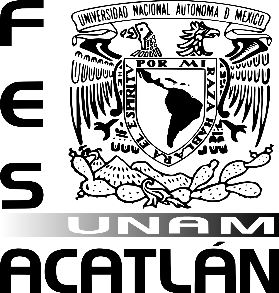
\includegraphics[width=0.15\textwidth]{../auxiliary/assets/fes.png}

        \vspace*{5cm}
        \LARGE
        \textbf{\titulo}

        \vspace{1cm}
        \large
        Camargo Badillo Luis Mauricio \\
        \vspace{1.5cm}

        \vfill

        \vspace{0.5cm}
        Audiciones Fase 3 \\
        \textbf{Programa de Inducción a Matemáticas Aplicadas y Computación}\\
    \end{center}
\end{titlepage}


\tableofcontents
\newpage

Recordemos que una \textit{ecuación diferencial} es una ecuación que relaciona una (o más) funciones con sus derivadas. Estas ecuaciones son de gran utilidad, pues nos ayudan a modelar muchos fenómenos naturales, el objeto de estudio de muchas disciplinas como la física, la ingeniería, la química, la biología, la astronomía, etc.; las ecuaciones diferenciales también modelan otros fenómenos de la economía y otras ciencias matemáticas. Es por esta razón por la que la resolución de ecuaciones diferenciales es un área de tanto interés en el mundo actual.

Usualmente, al tener una ecuación diferencial, el objetivo es encontrar la función (o las funciones) que la satisfagan. No obstante, dependiendo de la complejidad de la ecuación y de su forma, puede ser difícil o incluso imposible encontrar la solución exacta y explícita de forma analítica, un problema que se presenta sin importar si buscamos la solución manualmente o le asignamos la tarea a una computadora. De hecho, son bastantes las aplicaciones que involucran ecuaciones diferenciales cuya solución no se puede obtener de forma analítica; las ecuaciones que definen la forma del ala de un avión son un ejemplo.

Es por esta problemática por lo que nos apoyamos de los métodos numéricos para resolver este tipo de ecuaciones diferenciales. Recordemos que los métodos numéricos son técnicas que nos ayudan a aproximar procesos matemáticos y que se han vuelto especialmente populares luego del \textit{boom} en poder computacional que se ha experimentado en las últimas décadas; la resolución de esta clase de ecuaciones diferenciales son tan solo una de las muchas aplicaciones de los métodos numéricos.

Evidentemente, dada la naturaleza de los métodos numéricos, no tendremos una solución exacta como la analítica, pero ciertamente podemos tener una solución lo suficientemente cercana como para poder confiar en ella. En el mundo actual, podemos constatar que las soluciones obtenidas son perfectamente válidas: miles de aviones vuelan todos los días a pesar de que las ecuaciones que modelan la aerodinámica deben ser resueltas numéricamente.

Los \textbf{métodos de Runge-Kutta} son algunos de los métodos numéricos más ampliamente utilizados para la resolución de estas ecuaciones diferenciales, dado un problema de valor inicial. Estos métodos proporcionan soluciones más precisas que aquellas dadas por otros métodos numéricos más sencillos, como el método de Euler. A lo largo de este documento, se estará dando un panorama general de estos métodos, sus diferentes tipos y cómo utilizarlos, cerrando con una aplicación.

\section{Introducción a los Métodos de Runge-Kutta}

Los métodos de Runge-Kutta son una familia de métodos numéricos iterativos desarrollados por los matemáticos alemanes Carl Runge y Wilhelm Kutta alrededor de los inicios del siglo XX.\@

Estos métodos tienen como objetivo aproximar la solución de un problema de valor inicial que involucra una ecuación diferencial \textit{ordinaria}, especialmente cuando se trata de aquellos cuya solución analítica es difícil o imposible de obtener, como ya fue mencionado en la introducción de este texto. Debido a su relativamente rápida convergencia en relación a otros métodos, los métodos de Runge-Kutta son ampliamente preferidos, a pesar de que son computacionalmente más demandantes,

De forma similar a otros métodos numéricos utilizados para las ecuaciones diferenciales, los métodos de Runge-Kutta son iterativos, lo que quiere decir que una primera estimación es utilizada para obtener una segunda más precisa y así sucesivamente.

\section{Método de Runge-Kutta de Grado 4}

El método más utilizado de los Runge-Kutta es el de grado 4, frecuentemente conocido como «RK4»; incluso algunas veces es simplemente llamado \textit{el} método de Runge-Kutta.

\subsection{Funcionamiento de RK4}

Sea la siguiente ecuación diferencial:
\[
	\frac{dy}{dt} = f(t,y)
\]
…con la condición de valor inicial:
\[
	y(t_0) = y_0
\]
Aquí conocemos \(f\) y las condiciones inicales \(t_0, y_0\), deseando aproximar a \(y\), una función desconocida sobre \(t\). Utilizaremos el método RK4 para obtener esta aproximación.

Antes que nada, debemos:
\begin{itemize}
	\item Definir el intervalo para \(t\) sobre el cual estaremos aproximando la solución.
	\item Definir el tamaño \(h\) de los pasos por iteración que estaremos tomando sobre ese intervalo.
\end{itemize}
El número de iteraciones que realizaremos dependerá de la razón entre el intervalo para \(t\) y el tamaño \(h\) que elegimos anteriormente.

Comenzamos definiendo los dos valores más importantes que se estarán determinando durante cada iteración \(n \in [0, 1, 2, \dots]\):
\begin{align*}
	y_{n+1} &= y_{n} + \frac{h}{6} \left( k_{1} + 2k_{2} + 2k_{3} + k_{4} \right) \\[0.5em]
	t_{n+1} &= t_{n} + h
\end{align*}
Es en la definición de \(y_{n+1}\) que se nos presentan los valores \(k_{1}, k_{2}, k_{3}, k_{4}\), que son los que caracterizan al método RK4 y donde realizaremos la mayor cantidad de cálculos involucrados. Estos cuatro valores se definen para cada iteración \(n\) como:
\begin{align*}
	k_{1} &= f(t_{n}, y_{n}) \\
	k_{2} &= f \left( t_{n} + \frac{h}{2}, y_{n} + h \frac{k_{1}}{2} \right) \\
	k_{3} &= f \left( t_{n} + \frac{h}{2}, y_{n} + h \frac{k_{2}}{2} \right) \\
	k_{4} &= f(t_{n} + h, y_{n} + hk_{3})
\end{align*}

\subsection{Visualización de RK4}

Puede que hasta el momento la descripción anterior del método de Runge-Kutta de grado 4 (RK4) haya parecido bastante abstracta, pero describámosla y visualicémosla para que su funcionamiento quede más claro.

\begin{figure}[H]
	\centering
	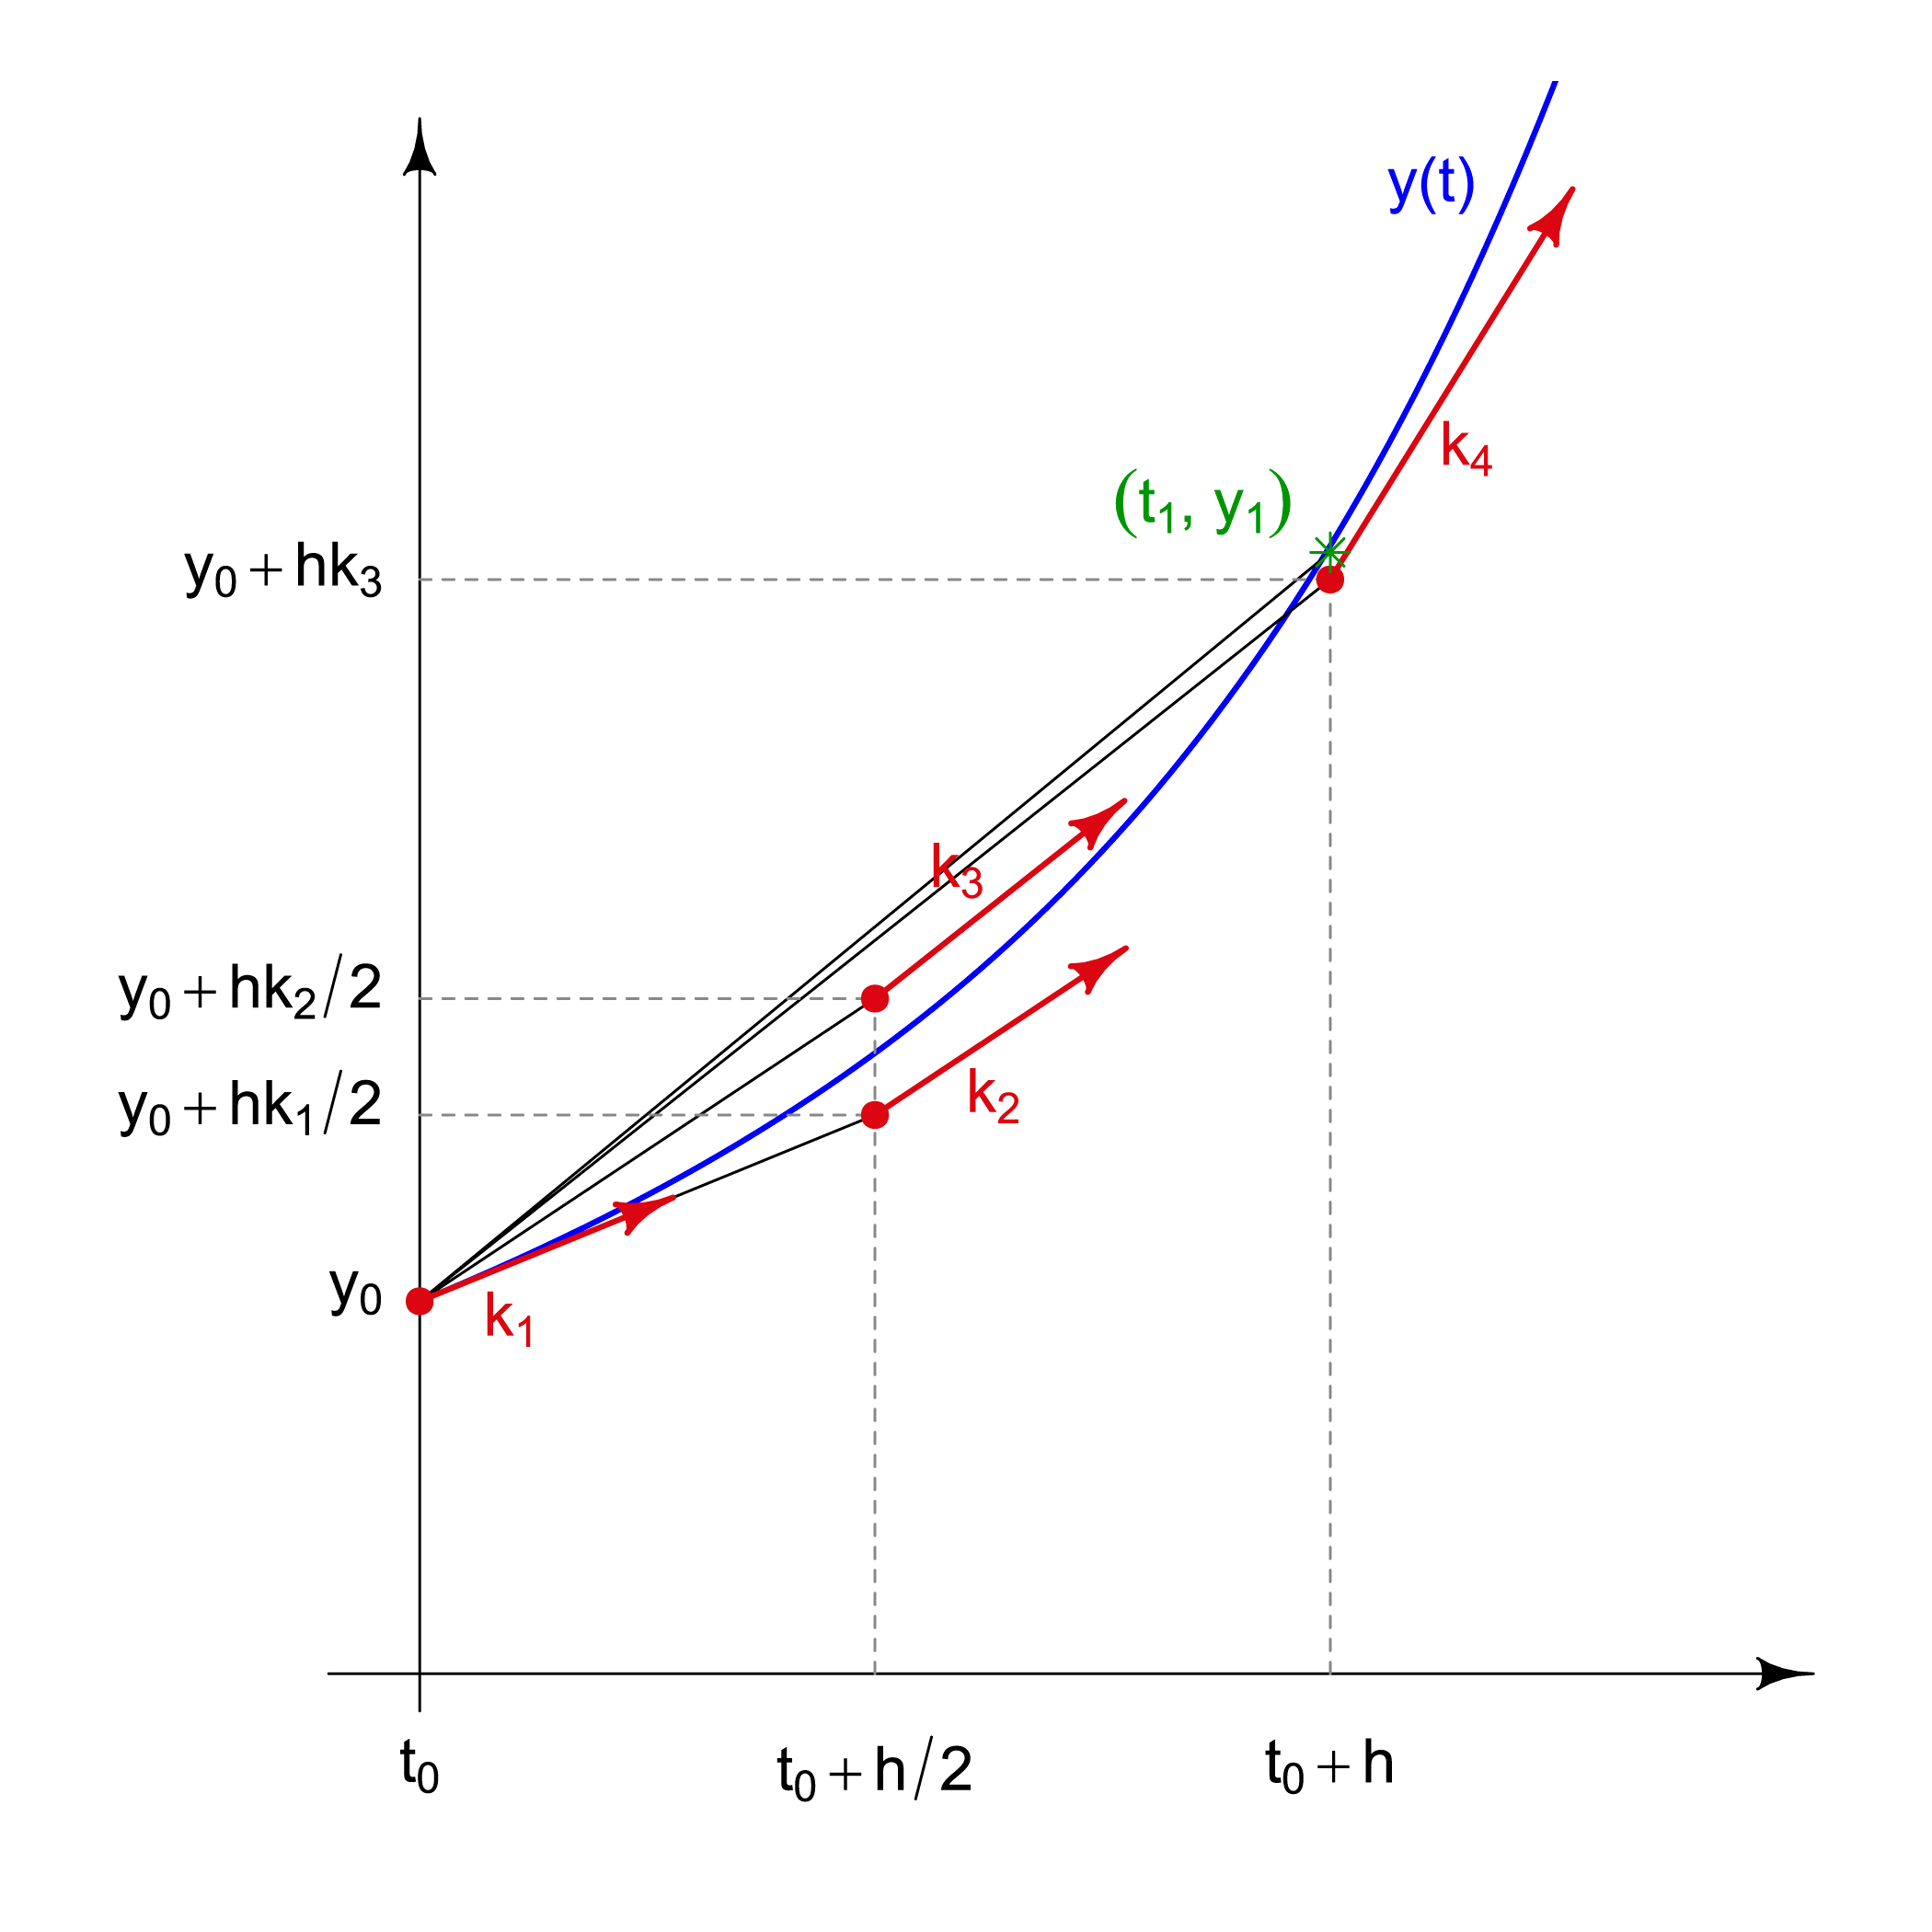
\includegraphics[scale=0.6]{Runge-Kutta_slopes.png}
	\caption{Aproximación de la solución a \(\frac{dy}{dt} = y + t^{3}\) con \(y_{0}\) y un intervalo para \(t\) arbitrarios. En azul, la solución exacta; en rojo, las pendientes correspondientes a los valores \(k_{i}\); en verde, uno de los puntos de la solución, que corresponde a la aproximación obtenida durante la primera iteración con paso \(h\).}
	\label{fig:slopes}
\end{figure}
La figura~\ref{fig:slopes} representa el funcionamiento de RK4 para la obtención de la solución a la ecuación diferencial \(\frac{dy}{dt} = y + t^{3}\) bajo la condición \(y(t_{0}) = y_{0}\), con \(y_{0}\) y el intervalo para \(t\) arbitrarios.

La obtención analítica de la solución exacta para esta ecuación diferencial es, de hecho, posible y es por ello por lo que pudo ser trazada como la línea azul, por lo que estrictamente hablando no es necesaria la implementación de un método numérico para obtenerla. Sin embargo, se ha utilizado simplemente para ejemplificar y visualizar el funcionamiento del método RK4.

\subsubsection{Pendientes a lo Largo del Intervalo}

Lo primero que notamos es que los valores \(k_{i}\) representan pendientes. Si regresamos a su definición en la sección anterior, notamos que son simplemente evaluaciones de \(f(t,y)\) en valores concretos de \(t\) y \(y\), y que la ecuación diferencial de la que partimos es \(\frac{dy}{dt} = f(t, y)\), por lo que la razón de ser de este resultado se vuelve evidente.

Analizando un poco más las definiciones de estas \(k_{i}\), y con ayuda de la figura~\ref{fig:slopes}, notaremos también que estas pendientes no son del todo arbitrarias:
\begin{itemize}
	\item \(k_{1}\) es la pendiente al inicio del intervalo.
	\item \(k_{2}\) es la pendiente en el punto medio del intervalo (de ahí que involucre \(\frac{h}{2}\)), apoyándose de \(k_{1}\).
	\item \(k_{3}\), similar a \(k_{2}\), es la pendiente en el punto medio del intervalo, pero esta vez apoyándose de \(k_{2}\).
	\item \(k_{4}\) es la pendiente al final del intervalo
\end{itemize}

\subsubsection{Aproximación Obtenida}

Al final de cada iteración \(n\) obtenemos \(y_{n+1}\), que no es más que la aproximación de \(y(t_{n+1})\) según el método. Notemos que este valor es determinado por la \(y_{n}\) actual correspondiente a la iteración, sumada con una media ponderada de cuatro incrementos, cada uno correspondiendo al producto de las cuatro pendientes anteriormente descritas por la longitud del paso \(h\).

\section{Forma General de los Métodos de Runge-Kutta}

\section{Aplicaciones de los Métodos de Runge-Kutta}

\section{Conclusión}

\end{document}
